

\begin{frame}{historique des événements liés à la réglementation du système bancaire}
\begin{table}[htbp]
    \centering
    \begin{tabular}{|c|p{4cm}|p{4cm}|}
        \hline
        \textbf{Année} & \textbf{Événement} & \textbf{Conséquences} \\
        \hline
        1974 & Faillite de la Herstatt Bank & Crise financière en Europe \\
             & Création du Comité de Bâle & Établissement de normes de régulation \\
        \hline
        1975 & Concordat de Bâle & Exigences minimales de fonds propres \\
        \hline
        1995-1998 & Crise mexicaine, crise asiatique & Élaboration de Bâle II \\
        \hline
        2007-2008 & Crise des subprimes, faillite de Lehman Brothers & Élaboration de Bâle III \\
        \hline
        2017 & Finalisation de Bâle III & Mise en œuvre des accords de Bâle III \\
        \hline
    \end{tabular}
   % \caption{Chronologie des crises du système bancaire}
    %\label{tab:crises_bancaires}
\end{table}
\end{frame}

\begin{frame}{La création du Comité de Bâle}
    \begin{figure}[h]
        \centering
        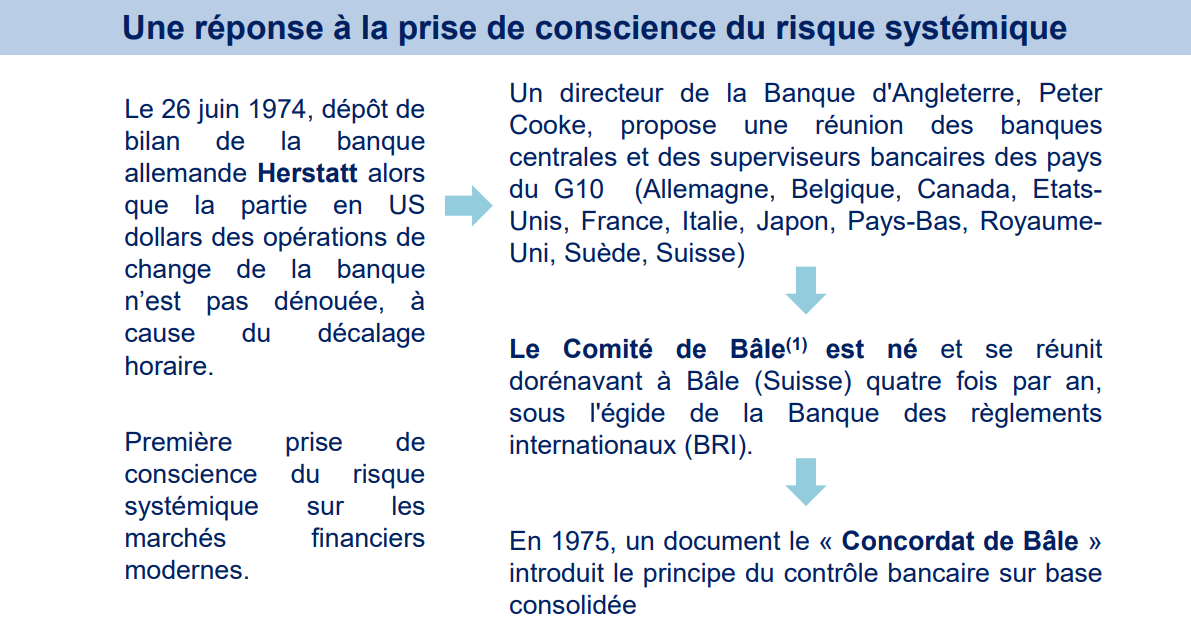
\includegraphics[scale=0.45]{Frames/Les Accords de Bale/p2.png}
        %\caption{Une réponse à la prise de conscience du risque systémique}
        %\label{fig:accords_bale_2}
    \end{figure}
\end{frame}


\begin{frame}{Le 1er accord de Bâle, dit ratio Cooke}
    \begin{figure}[h]
        \centering
        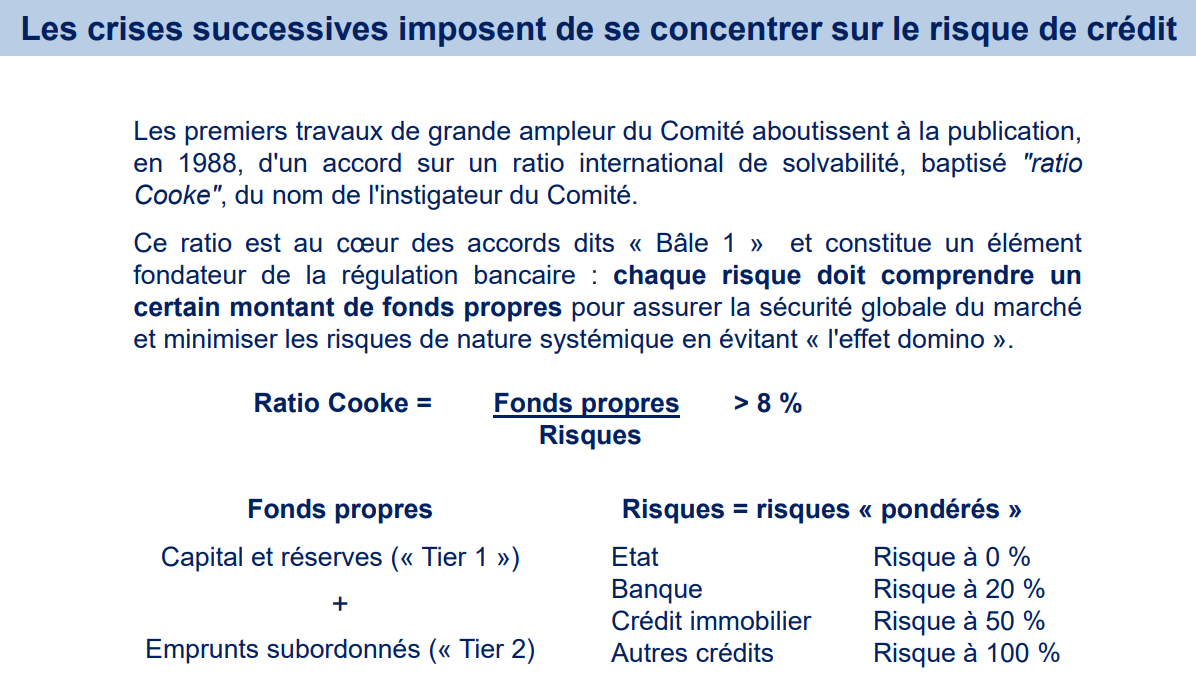
\includegraphics[scale=0.45]{Frames/Les Accords de Bale/p3.png}
       % \caption{Les crises successives imposent de se concentrer sur le risque de crédit}
        %\label{fig:accords_bale_2}
    \end{figure}
\end{frame}


\begin{frame}{Bâle 2 : les 3 piliers de la régulation bancaire}
    \begin{figure}[h]
        \centering
        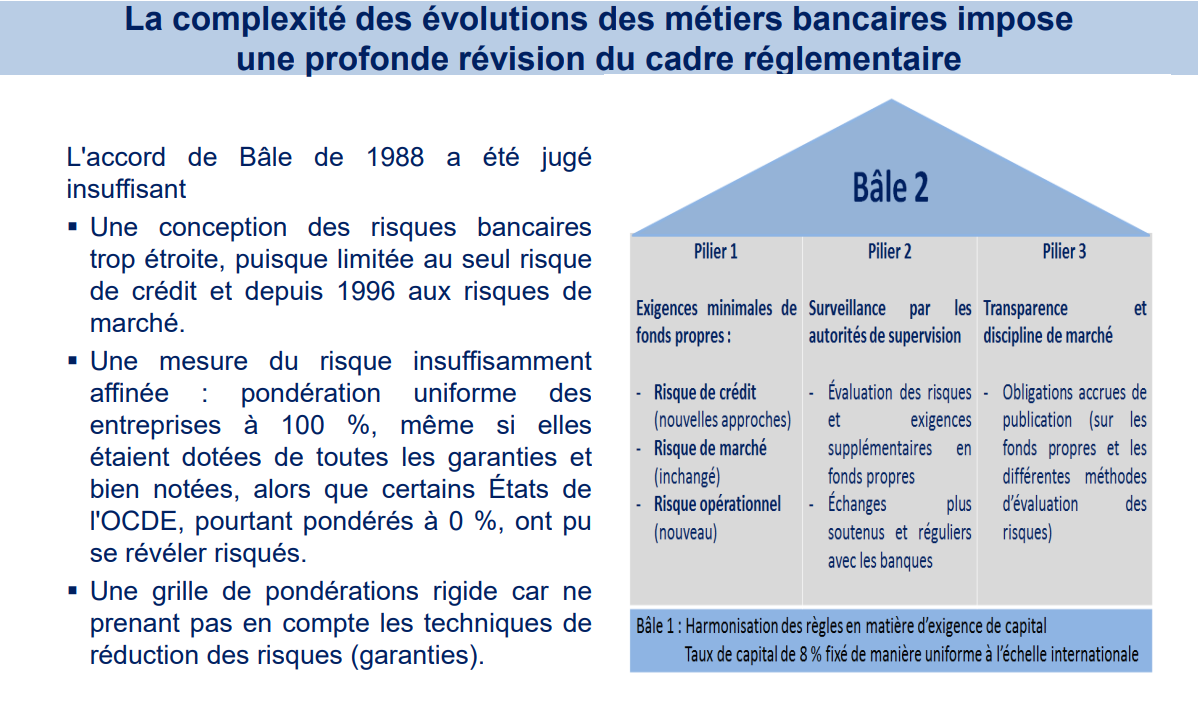
\includegraphics[scale=0.47]{Frames/Les Accords de Bale/p4.png}
        %\caption{La complexité des évolutions des métiers bancaires}
        %\label{fig:accords_bale_2}
    \end{figure}
\end{frame}


\begin{frame}{Bâle 3 : répondre à la crise de 2007/2008 et 2010}
    \begin{figure}[h]
        \centering
        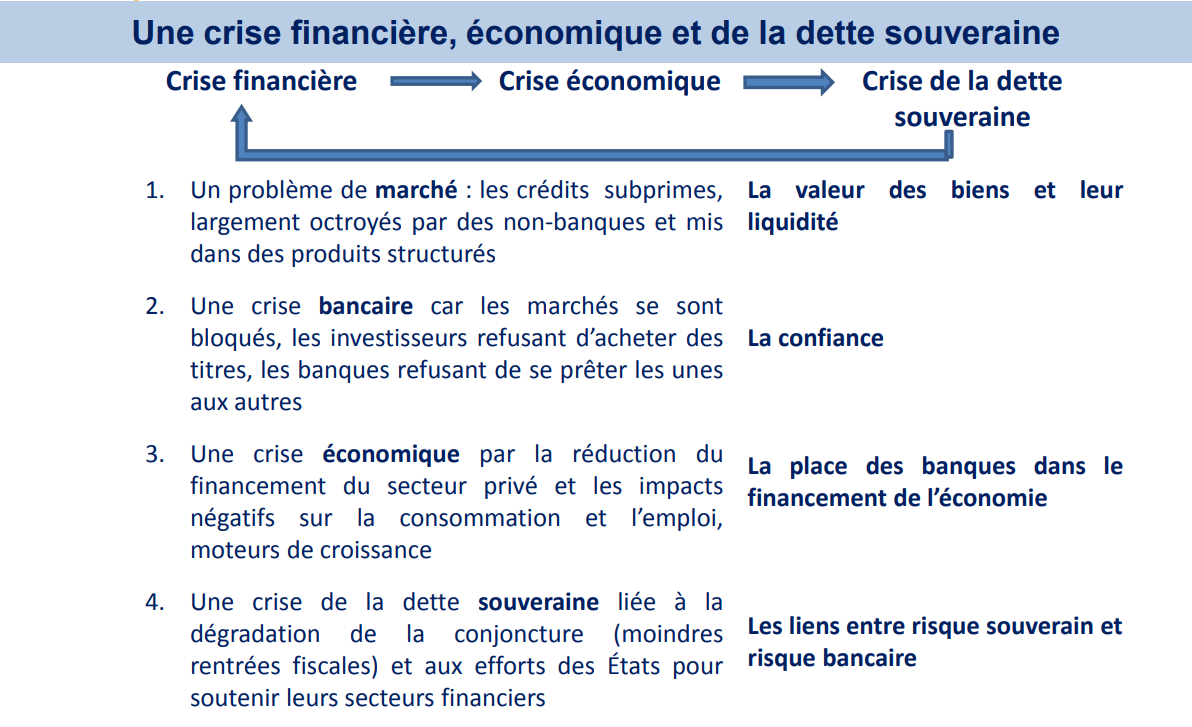
\includegraphics[scale=0.4]{Frames/Les Accords de Bale/b3.png}
        %\caption{Une crise financière, économique et de la dette souveraine}
        %\label{fig:accords_bale_2}
    \end{figure}
\end{frame}







\begin{frame}{Bâle 3 : répondre à la crise de 2007/2008 et 2010}
    \begin{figure}[h]
        \centering
        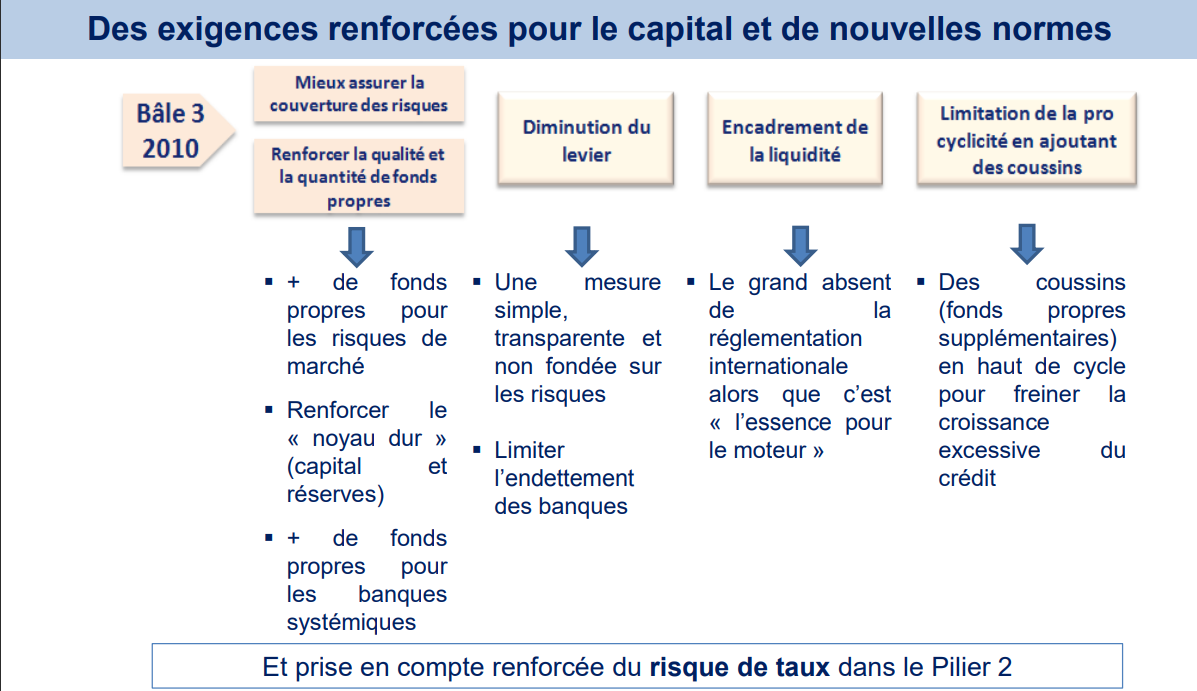
\includegraphics[scale=0.43]{Frames/Les Accords de Bale/b6.png}
        %\caption{Quatre normes quantitatives au lieu d’une seul }
        %\label{fig:accords_bale_2}
    \end{figure}
\end{frame}




\begin{frame}{Finalisation de Bâle 3}
    \begin{figure}[h]
        \centering
        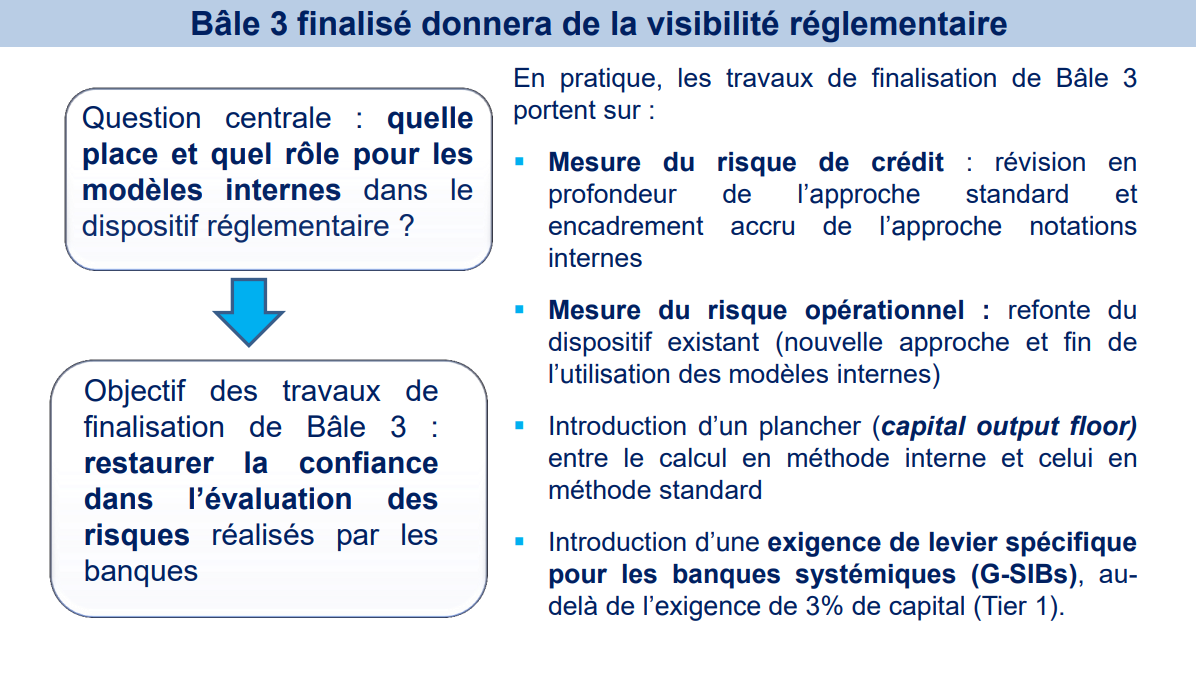
\includegraphics[scale=0.43]{Frames/Les Accords de Bale/b7.png}
       % \caption{Combler les insuffisances et les défauts  de la réglementation Bâle2 }
        %\label{fig:accords_bale_2}
    \end{figure}
\end{frame}